\chapter{Planificación del proyecto}\label{capPlanificacion}
A continuación se realiza una explicacion extensiva de la planificación inicial y final de nuestro proyecto.





\section{Planificación temporal inicial}\label{sec:planTemporalInicial}

En la figura \ref{fig:ganttInicial} se puede observar el diagrama de Gantt con la planificación inicial de este proyecto.
\begin{figure}[h!]
    \centering
    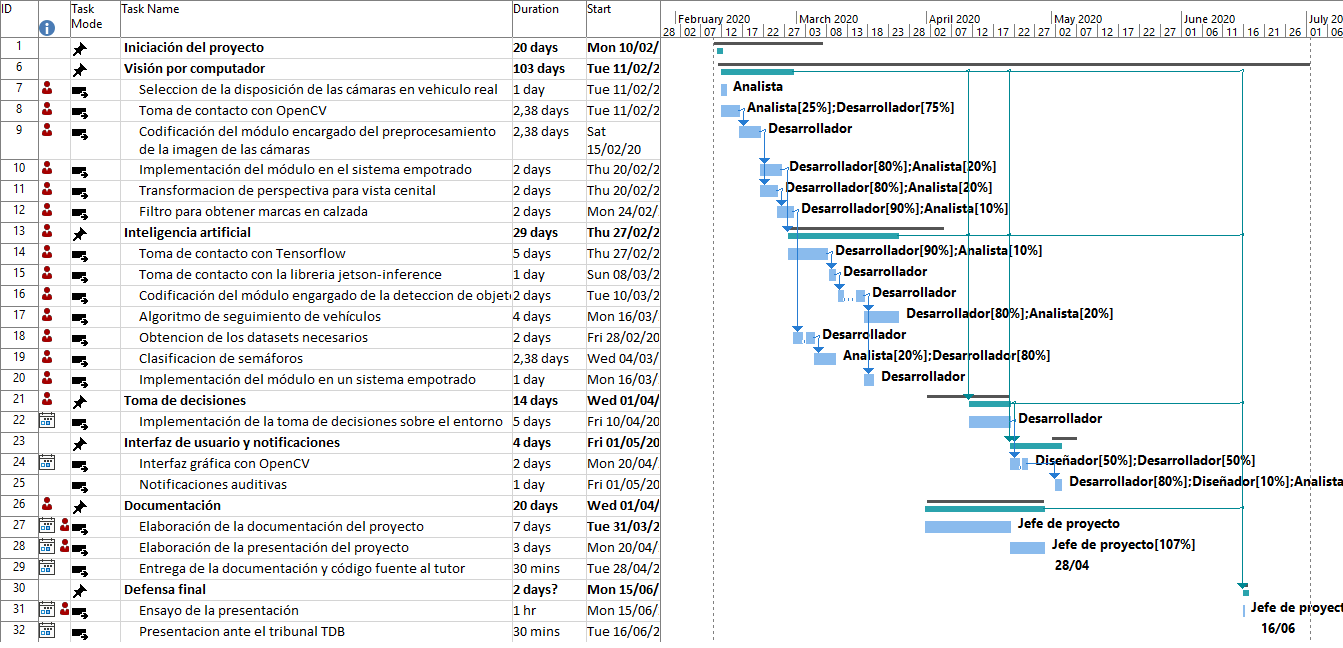
\includegraphics[width=0.9\linewidth]{img/Inicial/gantt-inicial.png}
    \caption{Diagrama de Gantt de la planificación inicial}
    \label{fig:ganttInicial}    
\end{figure}

\section{Planificación financiera inicial}\label{sec:planFinancieroInicial}
En cuanto a la planificación financiera inicial, se esperaba que el desarrollo del proyecto costase aproximadamente unos 20.125\euro y que tuviese una evolución como la que se puede observar en la figura \ref{fig:gastosInicial}
\begin{figure}[h!]
    \centering
    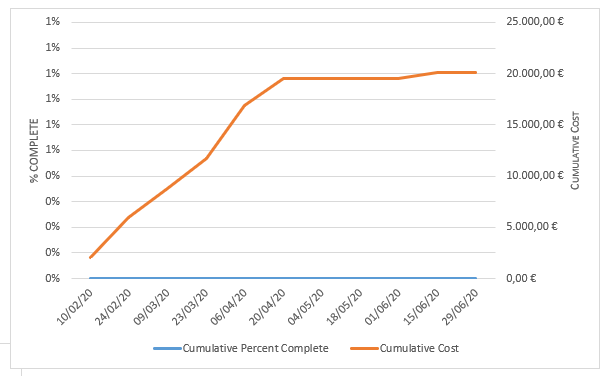
\includegraphics[width=0.7\linewidth]{img/Inicial/costes.PNG}
    \caption{Diagrama de planificación de gastos inicial}
    \label{fig:gastosInicial}    
\end{figure}


\section{Retrasos provocados por diversos motivos y cambios en el trabajo}

A pesar de haber planificado la realización de las tareas del proyecto de acuerdo a lo descrito en los apartados anteriores, a medida que se iba realizando el proyecto se fueron encontrando diversas dificultades que impidieron el seguimiento de la planificación.

La primera de ellas fue el gran retraso que se produjo tras la imposibilidad de acceder al hardware de desarrollo debido al estado de alarma nacional decretado debido a la crisis sanitaria global provocada por el virus SARS-CoV-2.
Tras los retrasos provocados por la falta del hardware se decidió aplazar la fecha de entrega de este trabajo a la siguiente convocatoria. 

Durante el periodo de cuarentena también se decidió migrar la ejecución del sistema desde un vehículo real a un simulador ya que, debido a la situación, depender de la conducción de un vehículo real no parecía ser una opción razonable.

Finalmente otro de los problemas encontrados durante la elaboración del proyecto fue el cambio de dos a un único autor, lo que supuso una mayor carga de trabajo ya que, como se ha observado, incluso la planificación inicial del trabajo se trataba de una planificación para 2 personas.


\section{Planificación temporal final} \label{sec:planTemporalFinal}
Finalmente, tras los cambios, la planificación temporal al finalizar el trabajo coincide con la que se puede observar en la figura \ref{fig:ganttfinal}.
\begin{figure}[t]
    \centering
    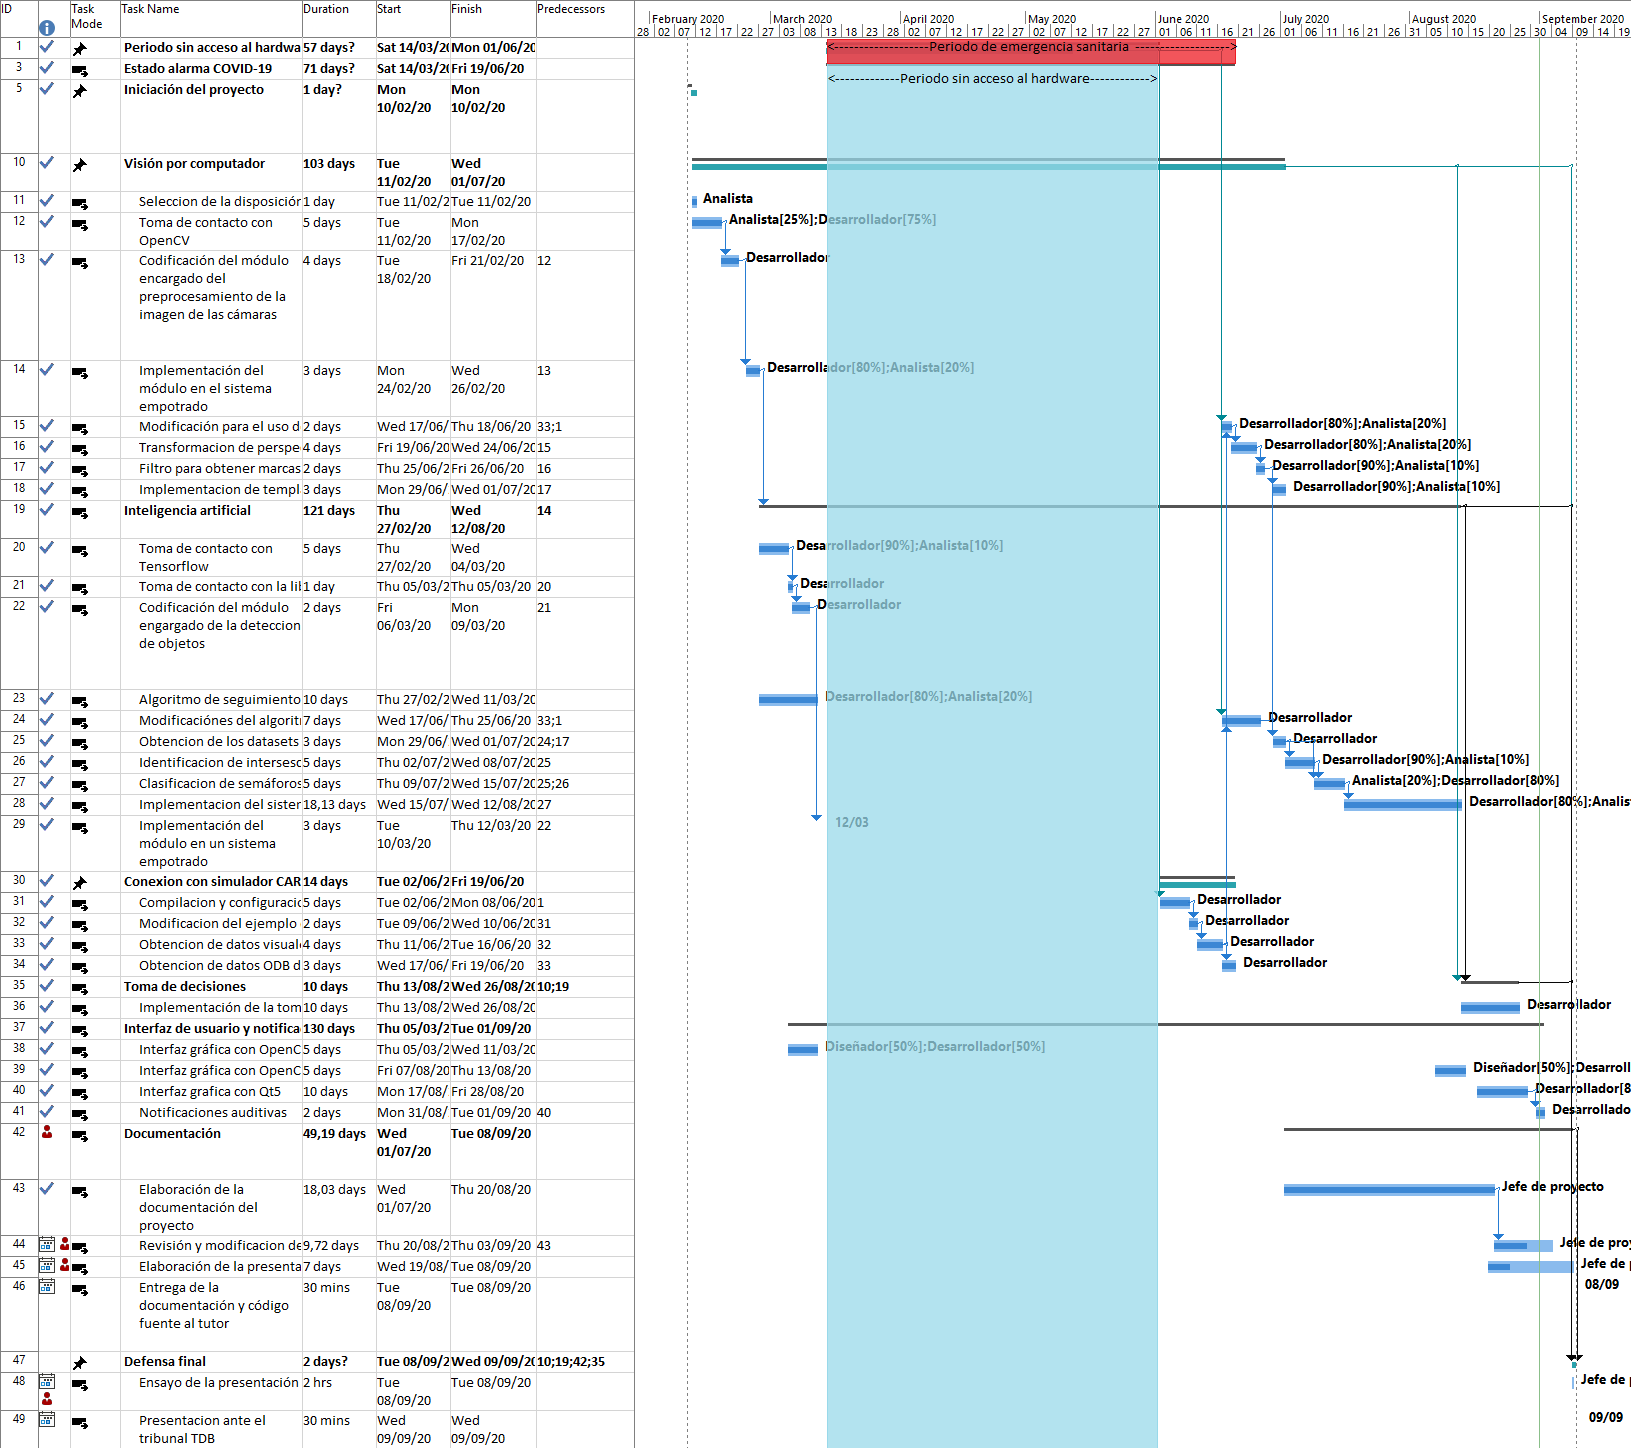
\includegraphics[width=\linewidth]{img/Final/gantt.png}
    \caption{Diagrama de Gantt de la planificación final}
    \label{fig:ganttfinal}    
\end{figure}


\section{Planificación financiera final} \label{sec:planFinancieroFinal}
La planificación financiera final del trabajo se ha visto modificada para coincidir con la nueva planificación.
Tal y como se puede comprobar en la figura \ref{fig:gastosFinal} la cifra final asciende a 39.546 \euro. 
\begin{figure}[h!]
    \centering
    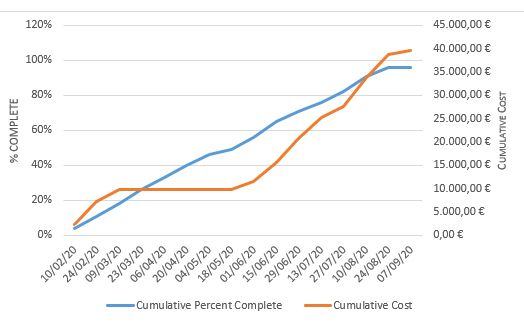
\includegraphics[width=0.7\linewidth]{img/Final/costes.PNG}
    \caption{Diagrama de planificación de gastos final}
    \label{fig:gastosFinal} 
\end{figure}



\section{Precios utilizados}
Los precios utilizados para el cálculo de la planificación financiera han sido un redondeo de los precios medios que se pueden observar en \cite{preciosInformatica}.
A modo informativo, en la tabla \ref{tab:precios} se pueden observar cuales han sido estas cantidades.

\begin{table}[h!]
    \centering
    \begin{tabular}{@{}ll@{}}
    \toprule
    Posición                                  & Salario/hora                         \\ \midrule
    Jefe de proyecto                          & 37 \euro                                 \\
    Analista                                  & 30 \euro                                  \\
    Desarrollador                             & 25 \euro                                  \\
    Diseñador                                 & 31 \euro                                  \\ \bottomrule
    \end{tabular}
    \caption{Precios utilizados para el cálculo de la planificación financiera}
    \label{tab:precios}
\end{table}




\section{Estudio de mercado} \label{sec:estudioDeMercado}
\subsection{Clientes potenciales} \label{sec:clientesPotenciales}

Los principales clientes potenciales de este sistema serán las empresas automovilísticas que no dispongan de un equipo centrado en el desarrollo de sistemas de conducción y que esten dispuestos a considerar una opción como la nuestra.

\subsection{Plan de comercialización} \label{sec:planComercializacion}

Teniendo en cuenta el precio final del sistema desarrollado y considerando lo que aportaría a una empresa automovilística, para la cual los precios de los extras suelen ser abismales creemos que el precio final al que se debería vender un sistema parecido al desarrollado sería de 50000 \euro, lo que nos proporcionaría un beneficio de 10454 \euro. Por otra parte, para la empresa el precio de este sistema sería bastante competitivo. Si Suponemos que un acuerdo con NVIDIA le permitiría obtener el hardware a un precio reducido de 500 \euro podrían recuperar la inversión en apenas la venta de 100 vehículos si se vende nuestro software en un paquete de 1000 \euro.